
\documentclass[table]{eecslides}

% \usecolortheme{RimouskiDark}

\usepackage[english]{babel}
\usepackage{lipsum}
\usepackage{graphicx}
\usepackage{caption}
\usepackage{hyperref}
\usepackage{xcolor}
\usepackage[round,authoryear]{natbib}
\usepackage[protrusion=true,expansion=true]{microtype}
\usepackage{xcolor}
\usepackage{tabularx}

\setlength{\extrarowheight}{3pt}

\title[]{Data conservation - Perspectives, issues and solutions.}
\author[]{\color{white}  Miranda Bryant and Steve Vissault}
\website{\color{white} s.vissault@yahoo.fr}
\institute[\color{white} UQAR]{\color{white} \textbf{Les midis numériques}}
\date{ \color{white} \today}

\setbeamersize{text margin left=1cm} 
\setbeamersize{text margin right=1cm} 
\setbeamersize{text margin top=0.1cm} 

\begin{document}

\begin{frame}[plain]
\titlepage
\end{frame}


%%%%%%%%%%%%%%%%
\section{Introduction}
%%%%%%%%%%%%%%%%

\begin{frame}{Introduction}{Context}

All biologists collect data during their career but most of them are using \alert{inapropriate files}, called \textit{"flat files"}, to long term storage:

\begin{itemize}
	\item  Open Office or Microsoft spreadsheet
	\item  text and CSV files
\end{itemize}

\textbf{Some risks attributes at those practices:} Overwriting file, lost the full dataset or some records.

\end{frame}

%%%%%%%%%%%%%%%%%%%%%%%%%%%%%%%%%%%%%%%%%%%%%%%%%%%%%%%%

\begin{frame}{Introduction}{Context}

\textbf{\alert{Some disadvantage of classic storage file (i. e. Excel)}}

\begin{enumerate}
	\item No dynamic query, only filters
	\item Large dataset could be messy
	\item Exportability : Files corrupted, plateform could be different between users
	\item Absence of fonctionnality on manage multiple users
\end{enumerate}

%% Basic question for the public: How many people generate a dynamic cross table on Excel and got twice the same word because the first one start by a capital letter and the second doesn't start by a capital letter ?

%% Define briefly what's a medata file ?

\end{frame}

%%%%%%%%%%%%%%%%%%%%%%%%%%%%%%%%%%%%%%%%%%%%%%%%%%%%%%%%

\begin{frame}{Introduction}{Why do something different ?}


\begin{columns}[c]
	\begin{column}{.50\paperwidth}
		\begin{figure}
			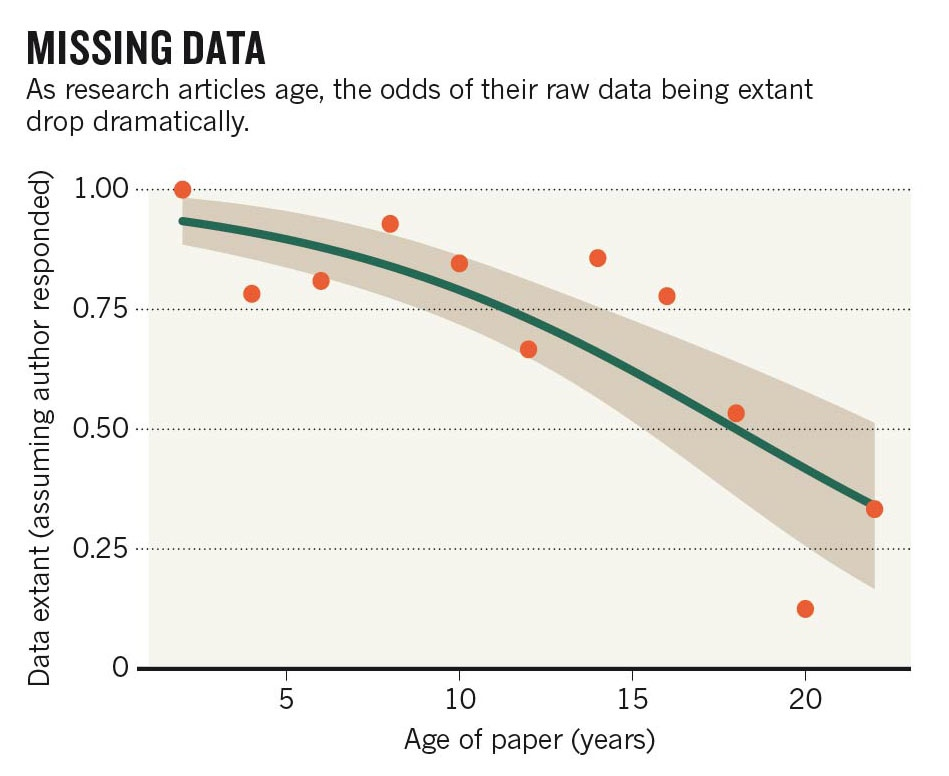
\includegraphics[width=.50\paperwidth]{Nature_fig.jpg}
		\end{figure}
	\end{column}
	\begin{column}{.4\paperwidth}
		 Data for almost all studies published just two years ago were still accessible, the chance of them being so \alert{fell by 17\% per year} \citep{Vines2013}
	\end{column}
\end{columns}

\end{frame}

%%%%%%%%%%%%%%%%%%%%%%%%%%%%%%%%%%%%%%%%%%%%%%%%%%%%%%%%


\begin{frame}{Introduction}{Why do something different ?}


\begin{columns}[c]
	\begin{column}{.50\paperwidth}
		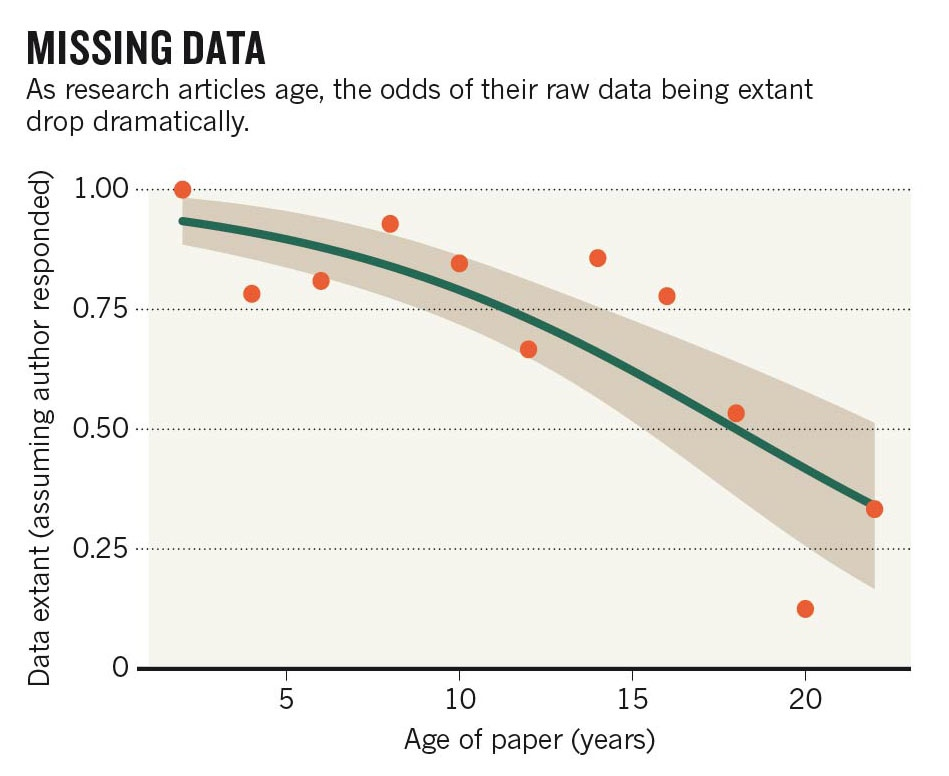
\includegraphics[width=.50\paperwidth]{Nature_fig.jpg}
	\end{column}
	\begin{column}{.4\paperwidth}
		\textbf{Why ?} Because researcher don't think about long term usability of storage data.
	\end{column}
\end{columns}

\end{frame}

%%%%%%%%%%%%%%%%%%%%%%%%%%%%%%%%%%%%%%%%%%%%%%%%%%%%%%%%

\begin{frame}{Introduction}{Why do something different ?}

\textbf{We need to keep focus on those points as a part of our biologist culture:}
	
	\begin{itemize}
		\item \alert{All datasets} containing specific information given a time and a location \alert{are usefull}.
		\item 80\% of datasets are built on \alert{public funding} \citep{Graham2013} and could be accessible publicly
		\item All datasets could be re-used, recycle or valorize (as the 3-R in waste management: Reduce, Reuse, Recycle) 
	\end{itemize}

	%% In this context, RDB could be a relevant solution for data in science

\end{frame}



%%%%%%%%%%%%%%%%%%%%%%%%%%%%%%%%%%%%%%%%%%%%%%%%%%%%%%%%

%%%%%%%%%%%%%%%%
\section{RDB}
%%%%%%%%%%%%%%%%

%%%%%%%%%%%%%%%%%%%%%%%%%%%%%%%%%%%%%%%%%%%%%%%%%%%%%%%%

\begin{frame}{Relational database}

\textbf{What is a Relational Database ?}
		 \begin{itemize}
			 \item A database is basically "tables" 
			\item A Table goes down a row of items and across many columns of attributes. The data can be organized into different tables.
			\item The tables have “relations” within and to each other
		 \end{itemize}

		\vfill

		\begin{center}
		 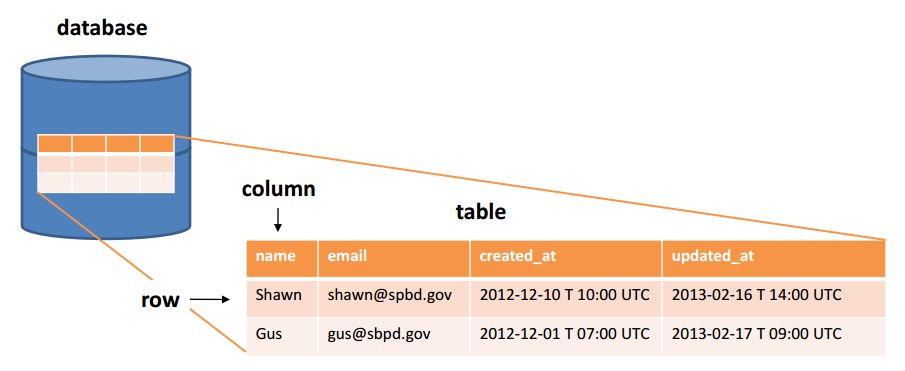
\includegraphics[width=.8\paperwidth]{relational-databases-for-dummies-fig1.png}
		\end{center}


	 %% Original text from Miranda: A Table goes down a row of items and across many columns of attributes (specific data descriptions). The data (along with new and different attributes) can be organized into different tables.

	%% Following the previous context, RDB seems to be a great and adapted solution to solve our problems.
\end{frame}

%%%%%%%%%%%%%%%%%%%%%%%%%%%%%%%%%%%%%%%%%%%%%%%%%%%%%%%%

\begin{frame}{Introduction}{Why is a relational database a relevant solution for this context ?}
	
	\textbf{Most of Relational databases include:}
	\begin{itemize}
		\item \alert{\textbf{Metadata}}: Authors, Year of creation, columns type and description
			\begin{itemize}
				\item You ensure the happiness of users after 10 years of database no-used
			\end{itemize}
		\item \alert{\textbf{Connectivity}}: Users can get a remote secure access to your own data
			\begin{itemize}
				\item You keep the control localy on your data and manage users
			\end{itemize}
		\item \alert{\textbf{Exportability:}} User can request data from different platforms and languages (i. e. C, C++, R etc...)
		\item \alert{\textbf{Provenence:}} Store modifications and user-related data changes that allow for “roll back” or “updates” to the data
	\end{itemize}

	%% Following the previous context, RDB seems to be a great and adapted solution to solve our problems.

\end{frame}

%%%%%%%%%%%%%%%%%%%%%%%%%%%%%%%%%%%%%%%%%%%%%%%%%%%%%%%%

\begin{frame}{Relational database}{What is a Relational Database ?}

\textbf{Four essential components:}
		 \begin{enumerate}
			 \item Row or Tuple : “A data set representing a single item” 
			\item Column: “A labeled element of a row” such an address, name, etc.
			\item Table: Contains data items in rows and columns
			\item Relationships : Links between tables and within table 
		 \end{enumerate}

	\textbf{Each components is embedded in a design diagram}

\end{frame}

%%%%%%%%%%%%%%%%%%%%%%%%%%%%%%%%%%%%%%%%%%%%%%%%%%%%%%%%
%%% Slide missing: Table employees table. See with Miranda if that could be extract from the case study (Tree table instead of using employees table)
%%%%%%%%%%%%%%%%%%%%%%%%%%%%%%%%%%%%%%%%%%%%%%%%%%%%%%%%

\begin{frame}{Relational database}{Table example}

\resizebox{\textwidth}{!}{
	\begin{figure}
		\begin{tabular}{cccccccccc}
			 \rowcolor{BlueBG}
			\hline
			ID PEP MES & YR & NO ARBRE & LATITUDE & LONGITUDE & DHPMM & CL DRAI & ESSENCE & ST CM2 & AGE\\
			\hline
			710AB& 1971 & 6 & 49.68091 & -74.96537 &  92 & NA & PIG &  66.48 & 39\\
			
			73096& 2005 & 52 & 47.88118 & -76.17882 & 125 & 30 & EPN & 122.72 & 93\\
			
			70004&2015 & 31 & 45,53753 & -71,08277 & 101 & NA & SAB &  80.12 & 47\\
			
			76013& 1992 & 2 &48,24704 &-69,67055 & 192 & 10 & PET & 289.53 & 52\\
			
			75010& 2007 & 49 & 48.43693 & -75.91256 & NA & 30 & NA &   0.00 & 18\\
			
			73008& 1980 & 13 & 47.50123 & -74.38295 & 187 &0 &RIR & 274.65 & 62\\
			
			72094& 1987 & 15 & 47.13014 & -76.02298 & 161 & NA & EPN & 203.58 & 55\\
			
			70094 & 2007 & 10 & 48.28338 & -71.73171 & 170 & 20 & & 226.98 & 68\\
			
			71006& 1992 & 25 & 47.32089 & -71.11494 & 162 & 20 & SAB & 206.12 & 45\\
			
			76095 & 2003 & 17 & 47.38095 & -71.72239 & 277 & 40 & SAB & 602.63 & 54\\
			\hline
		\end{tabular}
	\end{figure}}

\end{frame}


%%%%%%%%%%%%%%%%%%%%%%%%%%%%%%%%%%%%%%%%%%%%%%%%%%%%%%%%
%%%%%%%%%%%%%%%%
\section{Design components}
%%%%%%%%%%%%%%%%
%%%%%%%%%%%%%%%%%%%%%%%%%%%%%%%%%%%%%%%%%%%%%%%%%%%%%%%%

%%%%%%%%%%%%%%%%%%%%%%%%%%%%%%%%%%%%%%%%%%%%%%%%%%%%%%%%

\begin{frame}{Design components}{Wrong or messy informations}

\resizebox{\textwidth}{!}{
	\begin{figure}
		\begin{tabular}{cccccccccc}
			 \rowcolor{BlueBG}
			\hline
			ID PEP MES & YR & NO ARBRE & LATITUDE & LONGITUDE & DHPMM & CL DRAI & ESSENCE & ST CM2 & AGE\\
			\hline
			\cellcolor{red!50}710AB& 1971 & 6 & 49.68091 & -74.96537 &  92 & NA & PIG &  66.48 & 39\\
			
			73096& 2005 & 52 & 47.88118 & -76.17882 & 125 & 30 & EPN & 122.72 & 93\\
			
			70004& \cellcolor{red!50}2015 & 31 & 45,53753 & -71,08277 & 101 & NA & SAB &  80.12 & 47\\
			
			76013& 1992 & 2 & \cellcolor{red!50}48,24704 & \cellcolor{red!50}-69,67055 & 192 & 10 & PET & 289.53 & 52\\
			
			75010& 2007 & 49 & 48.43693 & -75.91256 & NA & 30 & NA &   0.00 & 18\\
			
			73008& 1980 & 13 & 47.50123 & -74.38295 & 187 & \cellcolor{red!50}0 & \cellcolor{red!50}RIR & 274.65 & 62\\
			
			72094& 1987 & 15 & 47.13014 & -76.02298 & 161 & NA & EPN & 203.58 & 55\\
			
			70094 & 2007 & 10 & 48.28338 & -71.73171 & 170 & 20 & \cellcolor{red!50} & 226.98 & 68\\
			
			71006& 1992 & 25 & 47.32089 & -71.11494 & 162 & 20 & SAB & 206.12 & 45\\
			
			76095 & 2003 & 17 & 47.38095 & -71.72239 & 277 & 40 & SAB & 602.63 & 54\\
			\hline
		\end{tabular}
	\end{figure}}

\end{frame}

%%%%%%%%%%%%%%%%%%%%%%%%%%%%%%%%%%%%%%%%%%%%%%%%%%%%%%%%

\begin{frame}{Design components}{Redundancy or calculated field}

\resizebox{\textwidth}{!}{
	\begin{figure}
		\begin{tabular}{cccccccccc}
			 \rowcolor{BlueBG}
			\hline
			ID PEP MES & YR & NO ARBRE &  \cellcolor{red!50} LATITUDE & \cellcolor{red!50}LONGITUDE & DHPMM & CL DRAI & ESSENCE & \cellcolor{red!50}ST CM2 & AGE\\
			\hline
			710AB& 1971 & 6 & 49.68091 & -74.96537 &  92 & NA & PIG &  66.48 & 39\\
			
			73096& 2005 & 52 & 47.88118 & -76.17882 & 125 & 30 & EPN & 122.72 & 93\\
			
			70004& 2015 & 31 & 45,53753 & -71,08277 & 101 & NA & SAB &  80.12 & 47\\
			
			76013& 1992 & 2 & 48,24704 & -69,67055 & 192 & 10 & PET & 289.53 & 52\\
			
			75010& 2007 & 49 & 48.43693 & -75.91256 & NA & 30 & NA &   0.00 & 18\\
			
			73008& 1980 & 13 & 47.50123 & -74.38295 & 187 & 0 & RIR & 274.65 & 62\\
			
			72094& 1987 & 15 & 47.13014 & -76.02298 & 161 & NA & EPN & 203.58 & 55\\
			
			70094 & 2007 & 10 & 48.28338 & -71.73171 & 170 & 20 &  & 226.98 & 68\\
			
			71006& 1992 & 25 & 47.32089 & -71.11494 & 162 & 20 & SAB & 206.12 & 45\\
			
			76095 & 2003 & 17 & 47.38095 & -71.72239 & 277 & 40 & SAB & 602.63 & 54\\
			\hline
		\end{tabular}
	\end{figure}}

\end{frame}

%%%%%%%%%%%%%%%%%%%%%%%%%%%%%%%%%%%%%%%%%%%%%%%%%%%%%%%%

\begin{frame}{Design components}{Normalization}

\textbf{What's normalization ?}

		\begin{itemize}
			\item Do not have the “one file” or “one table” mentality
			\item If you have redundancy in your table, you need to think about normalization (multiple table design)
			\item Stages of normalization 1-5 NF (Normal Forms) are the most commonly accepted
			\begin{itemize}
				\item These are “technical”, but they describe the stages a database development will go through
			\end{itemize}
		\end{itemize}

\end{frame}

%%%%%%%%%%%%%%%%%%%%%%%%%%%%%%%%%%%%%%%%%%%%%%%%%%%%%%%%

\begin{frame}{Design components}{A table contains keys}

\alert{\textbf{Table contain keys:}}
		 \begin{description}
			 \item [Primary Keys] A key that is unique to the table to help identify a record
			\item [Composite Keys] A key that combines two or more columns to create a unique key into the table
		\end{description}

\end{frame}

%%%%%%%%%%%%%%%%%%%%%%%%%%%%%%%%%%%%%%%%%%%%%%%%%%%%%%%%

\begin{frame}{Design components}{Relationships}

\textbf{Different type of relationship:}

		\begin{description}
			\item [1:1] Each key is linked with only one key in any other table
			\item [1:N] Each key in one table may be linked to many other keys in another table
			\item [N:N] One or more keys in a table can be linked to 0, 1, or many rows in another table
		\end{description}

\end{frame}



%%%%%%%%%%%%%%%%%%%%%%%%%%%%%%%%%%%%%%%%%%%%%%%%%%%%%%%%


\begin{frame}{Design components}{Last example not normalized}

\resizebox{\textwidth}{!}{
	\begin{figure}
		\begin{tabular}{cccccccccc}
			 \rowcolor{BlueBG}
			\hline
			ID PEP MES & YR & NO ARBRE & LATITUDE & LONGITUDE & DHPMM & CL DRAI & ESSENCE & ST CM2 & AGE\\
			\hline
			710AB& 1971 & 6 & 49.68091 & -74.96537 &  92 & NA & PIG &  66.48 & 39\\
			
			73096& 2005 & 52 & 47.88118 & -76.17882 & 125 & 30 & EPN & 122.72 & 93\\
			
			70004&2015 & 31 & 45,53753 & -71,08277 & 101 & NA & SAB &  80.12 & 47\\
			
			76013& 1992 & 2 &48,24704 &-69,67055 & 192 & 10 & PET & 289.53 & 52\\
			
			75010& 2007 & 49 & 48.43693 & -75.91256 & NA & 30 & NA &   0.00 & 18\\
			
			73008& 1980 & 13 & 47.50123 & -74.38295 & 187 &0 &RIR & 274.65 & 62\\
			
			72094& 1987 & 15 & 47.13014 & -76.02298 & 161 & NA & EPN & 203.58 & 55\\
			
			70094 & 2007 & 10 & 48.28338 & -71.73171 & 170 & 20 & & 226.98 & 68\\
			
			71006& 1992 & 25 & 47.32089 & -71.11494 & 162 & 20 & SAB & 206.12 & 45\\
			
			76095 & 2003 & 17 & 47.38095 & -71.72239 & 277 & 40 & SAB & 602.63 & 54\\
			\hline
		\end{tabular}
	\end{figure}}

\end{frame}

%%%%%%%%%%%%%%%%%%%%%%%%%%%%%%%%%%%%%%%%%%%%%%%%%%%%%%%%

\begin{frame}{Design components}{New and cleanest design}

\textbf{\alert{Need to be transform to the cleanest design without redundancy}}
\vspace{0.2cm}
	\begin{center}
		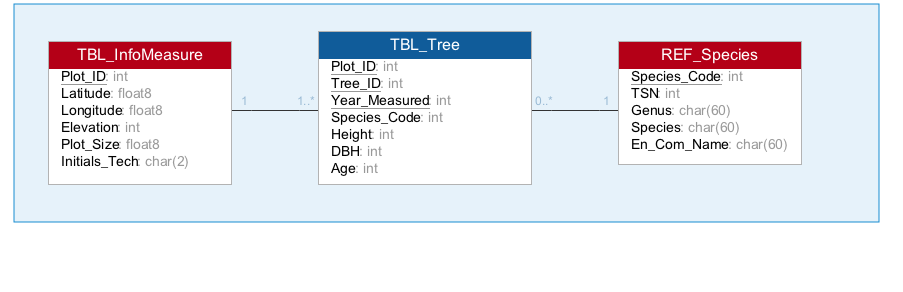
\includegraphics[width=0.8\paperwidth]{Ex1_pres_30Sept.png}
	\end{center}
\end{frame}

%%%%%%%%%%%%%%%%%%%%%%%%%%%%%%%%%%%%%%%%%%%%%%%%%%%%%%%%
%%%%%%%%%%%%%%%%
\section{RDB creation}
%%%%%%%%%%%%%%%%
%%%%%%%%%%%%%%%%%%%%%%%%%%%%%%%%%%%%%%%%%%%%%%%%%%%%%%%%

\begin{frame}{How to create this design ?}{SQL language}

\textbf{What does SQL mean?}
\begin{itemize}
	\item “Structured Query Language”
	\item This language was designed to be cross-platform to handle data in relational databases
	\item The International Organization for Standardization  the language in 1981
	\item Provides cross-platform consistence (most of the time)
\end{itemize}

\end{frame}

%%%%%%%%%%%%%%%%%%%%%%%%%%%%%%%%%%%%%%%%%%%%%%%%%%%%%%%%

\begin{frame}{How to create this design ?}{Create table}

\textbf{Table example creation:}
\begin{block}{SQL Code}
\begin{tabbing}
\texttt{CREATE TABLE "TBL-Tree" (\\
		\hspace{1cm} "Plot-ID" int NOT NULL,\\
		\hspace{1cm} "Tree-ID" int NOT NULL,\\
		\hspace{1cm} "Year-Measured" numeric(4) NOT NULL,\\
		\hspace{1cm} "Species-Code" char(3) NULL,\\
		\hspace{1cm} "Height" float8 NULL,\\
		\hspace{1cm} "DBH" numeric(5) NULL,\\
		\hspace{1cm} "Age" int NULL,\\
PRIMARY KEY ("Plot-ID", "Tree-ID", "Year-Measured") \\
);
}
\end{tabbing}
\end{block}

\end{frame}

%%%%%%%%%%%%%%%%%%%%%%%%%%%%%%%%%%%%%%%%%%%%%%%%%%%%%%%%

\begin{frame}{Basic manipulation}{Update}

\textbf{Simple to update to a large amount of data:}

\begin{block}{SQL Code}
\texttt{
UPDATE Tree-Species\\
	\hspace{1cm} SET genus-name = ‘Acer’\\
	\hspace{1cm} WHERE species-id = ’sacchaurm’;

}
\end{block}
Every update is recorded so if there is an error, it can be “rolled back” (undo)
\end{frame}

%%%%%%%%%%%%%%%%%%%%%%%%%%%%%%%%%%%%%%%%%%%%%%%%%%%%%%%%

\begin{frame}{QUICC-FOR Example}{Diagram}

\vspace{0.2cm}
	\begin{center}
		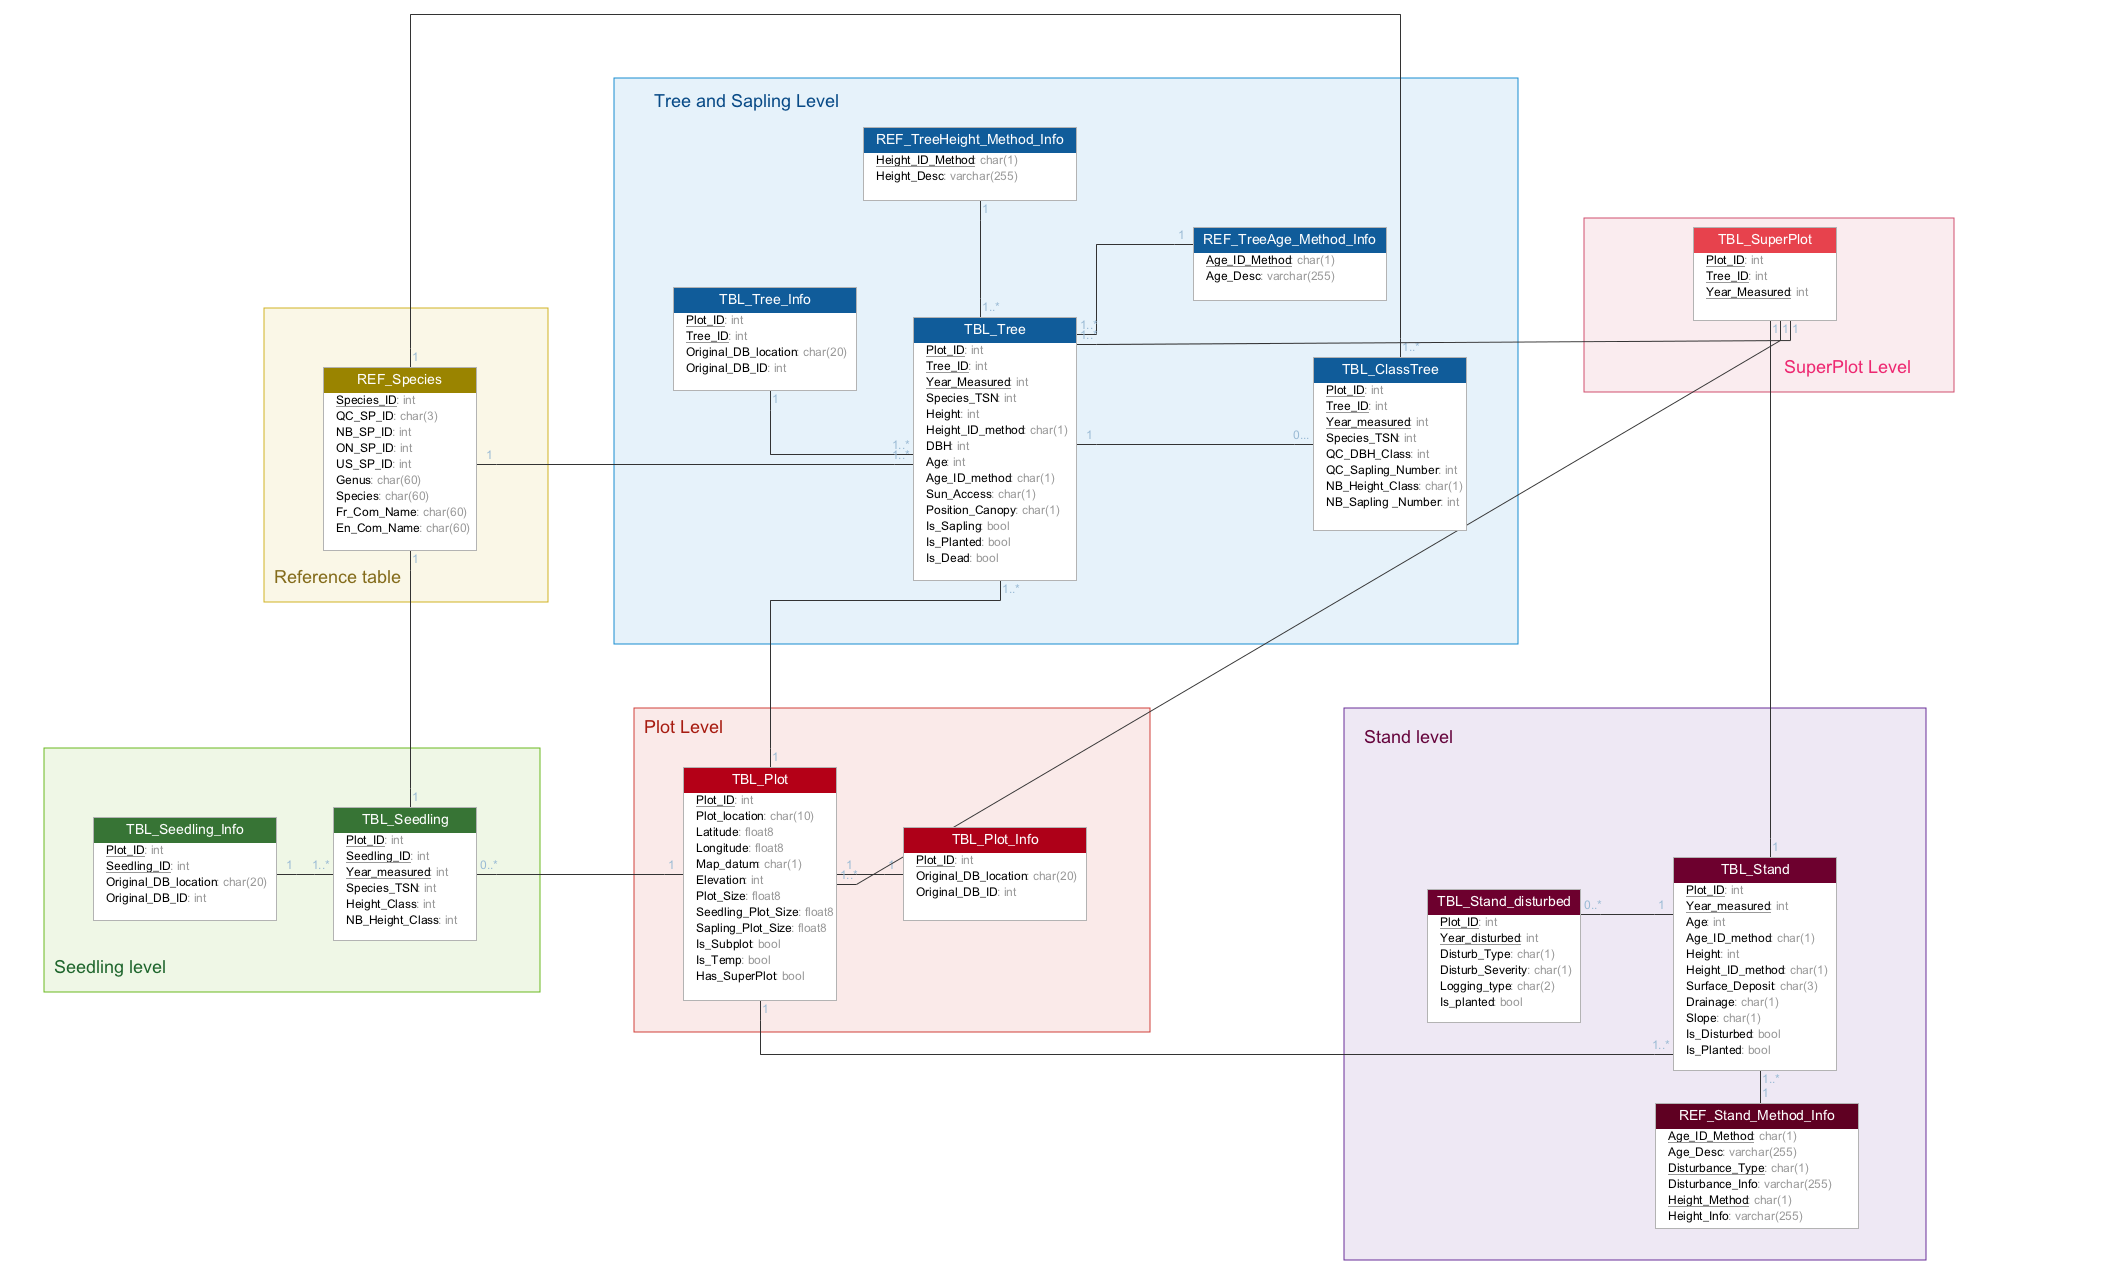
\includegraphics[width=0.8\paperwidth]{UML_QUICC.png}
	\end{center}

\end{frame}

%%%%%%%%%%%%%%%%%%%%%%%%%%%%%%%%%%%%%%%%%%%%%%%%%%%%%%%%

\begin{frame}{QUICC-FOR Example}{Diagram}

\textbf{QUICC FOR – A real-life example}
\begin{itemize}
	\item Data from two countries, over many years and many sources
	\item Data is in varying formats, all publicly available
	\item Created a normalized Database to store data
	\item Created a schema to merge and clean data
	\item Then worked to create a new schema that incorporates all data
\end{itemize}

\end{frame}

%%%%%%%%%%%%%%%%%%%%%%%%%%%%%%%%%%%%%%%%%%%%%%%%%%%%%%%%

\begin{frame}{Relationnal Database}{Disadvantages}

\textbf{Some disadvantages:}
	\begin{itemize}
		\item New system to learn that is not always intuitive
		\item System has to be setup to run a database
		\item Poor database design could be “worse” than a basic flat file
		\item Maintenance cost can be higher
	\end{itemize}

\end{frame}

%%%%%%%%%%%%%%%%%%%%%%%%%%%%%%%%%%%%%%%%%%%%%%%%%%%%%%%%

\begin{frame}{Relationnal Database}{Advantages}

\textbf{Some advantages:}
	\begin{itemize}
		\item “Coarse” data is never touched except by certain users
		\item Most users are always working on a query
		\item Data is publicly available but more secure 
		\item Multiple users can access data
		\item Log of all modifications with username
		\item Ability to “roll back” changes
		\item Size of data only limited by storage
		\item Secure, long distance connections to data
	\end{itemize}

\end{frame}


%%%%%%%%%%%%%%%%%%%%%%%%%%%%%%%%%%%%%%%%%%%%%%%%%%%%%%%%

\begin{frame}{Relationnal Database}{Exportability}

\textbf{Where can SQL be used ?}
	\begin{itemize}
			\item R
			\item Java
			\item C
			\item C++
			\item Perl
			\item Python
			\item .Net 
	\end{itemize}
\end{frame}




%%%%%%%%%%%%%%%%%%%%%%%%%%%%%%%%%%%%%%%%%%%%%%%%%%%%%%%%
%%%%%%%%%%%%%%%%
\section{Conclusion}
%%%%%%%%%%%%%%%%
%%%%%%%%%%%%%%%%%%%%%%%%%%%%%%%%%%%%%%%%%%%%%%%%%%%%%%%%

%%%%%%%%%%%%%%%%%%%%%%%%%%%%%%%%%%%%%%%%%%%%%%%%%%%%%%%%

\begin{frame}{Conclusion}{Metadata}

\textbf{What's metadata ?}
	\begin{description}
		\item [Defined:] “Metadata is data about data”
		\item [Examples:] Author, Journal Title, Edition, Publication Date or Tree description, date updated, collection date
	\end{description}
\end{frame}

%%%%%%%%%%%%%%%%%%%%%%%%%%%%%%%%%%%%%%%%%%%%%%%%%%%%%%%%

\begin{frame}{Conclusion}{Throughts}

\textbf{According to \citet{Goodman2014}, we need to keep focus on those points:}
	\begin{enumerate}
		\item Love your data and help others love it too
		\item Share your data online with a permanent identifier
		\item Conduct science with a particular level of reuse in mind
	\end{enumerate}
\end{frame}


%%%%%%%%%%%%%%%%
%% References
%%%%%%%%%%%%%%%%

\nocite{Poisot2013a}

\begin{frame}[allowsframebreaks]{References}
	\bibliographystyle{abbrvnat}
	\bibliography{/home/steve/Dropbox/Bibtex/OpenAccess}	
\end{frame}

\end{document}